\documentclass{beamer}

\mode<presentation> {
	\usetheme{Madrid}
	% \usecolortheme{default}
	% \setbeamertemplate{navigation symbols}{}  % 隐藏导航符号

	% \setbeamertemplate{footline}
	%若要删除所有幻灯片中的页脚,请取消注释此行
	
	%\setbeamertemplate{footline}[页码]
	%若要用简单的幻灯片计数替换所有幻灯片中的页脚,请取消注释此行
	
	%\setbeamertemplate{导航符号}{}
	%要删除所有幻灯片底部的导航符号,请取消注释此行
}

\usepackage{graphicx} % 允许包含图像
\usepackage{booktabs} % 允许在表中使用\toprule、\ midrule和\ bottomrule
\usepackage[UTF8,noindent]{ctexcap}  % 使用中文输入及显示
\usepackage[bookmarks=true]{hyperref}

%-----------------------------------
%	以下为正文
%-----------------------------------

\title[巧求周长(一)]{巧求周长(一)} 
% 简短标题显示在每张幻灯片的底部,完整标题仅在标题页上

\author{Zhuo}
\institute[] % 您的机构将出现在每张幻灯片的底部,可能是节省空间的简写
{
	% 会心升学 \\
	% \medskip
	% \textit{@163.com} % Your email address
}
\date{\today} % 日期,可以更改为自定义日期

\begin{document}
	\begin{frame}
		\vspace{-1cm}
		\begin{flushleft}
			
\includegraphics[width=1cm]{./pics/huixin_logo.png}
		\end{flushleft}
		\titlepage
	\end{frame}

	\begin{frame}
		\frametitle{目录}
		\tableofcontents % 在整个演示过程中,如果您选择使用\ section{}和\ submission{}命令,这些命令将自动打印在此幻灯片上,作为演示的概述
	\end{frame}
	
	%-----------------------------------
	%	开始创建PPT
	%-----------------------------------
	
	\section{第1讲\quad 计算}

\item {
    【乘法分配律】
    $(200+2)\times 5 + 5020$ 
    \ifshowSolution
        \fangsong\zihao{4}
        \\
        思路:改。2025

        正解: 
    \else
        \\ \\ \\
    \fi
}

% \item {
%     $(20+2)\times 5 + 2025$ 
%     \ifshowSolution
%         \fangsong\zihao{4}
%         \\
%         思路:2025

%         正解: 
%     \else
%         \\ \\ \\
%     \fi
% }

\item {
    【乘法分配律】
    $7\times 19 + 3\times 13\times 41 + 13\times 19$
    \ifshowSolution
        \fangsong\zihao{4}
        \\
        思路:改。2021;迎春杯四年级真题.pdf

        正解: 
    \else
        \\ \\ \\
    \fi
}

\item {
    【乘法分配律】
    $(18\times 23 - 24\times 17)\div 3 + 5$
    \ifshowSolution
        \fangsong\zihao{4}
        \\
        思路:

        正解: 
    \else
        \\ \\ \\
    \fi
}

\item {
    【乘法分配律】
    $(11\times 24 - 23\times 9)\div 3 + 3$
    \ifshowSolution
        \fangsong\zihao{4}
        \\
        思路:

        正解: 
    \else
        \\ \\ \\
    \fi
}

% \item {
%     【乘法分配律】
%     $7\times 17 + 3\times 13\times 43 + 13\times 17$
%     \ifshowSolution
%         \fangsong\zihao{4}
%         \\
%         思路:2021;迎春杯四年级真题.pdf

%         正解: 2017
%     \else
%         \\ \\ \\
%     \fi
% }

% \item {
%     $(9\times 8\times 7 + 6 - 5)\times 4 + 3 -2 +1$
%     \ifshowSolution
%         \fangsong\zihao{4}
%         \\
%         思路: 迎春杯四年级2022-试卷.pdf

%         正解: 2022
%     \else
%         \\ \\ \\
%     \fi
% }

\item {
    【乘法凑10】
    $12\times 25 + 16\times 15$
    \ifshowSolution
        \fangsong\zihao{4}
        \\
        思路:

        正解: 
    \else
        \\ \\ \\
    \fi
}

\item {
    【乘法凑10】
    $5\times 432\times 1 - 98 - 7\times 6$
    \ifshowSolution
        \fangsong\zihao{4}
        \\
        思路: 2020数学花园探秘笔试小中决赛D卷.doc

        正解: 2020
    \else
        \\ \\ \\
    \fi
}

\item {
    【加法凑10】
    $1+3+4+6+7+9+10 + 12$
    \ifshowSolution
        \fangsong\zihao{4}
        \\
        思路:

        正解: 
    \else
        \\ \\ \\
    \fi
}

\item {
    【乘法凑10】
    $210\times 6 - 52\times 5$
    \ifshowSolution
        \fangsong\zihao{4}
        \\
        思路:

        正解: 
    \else
        \\ \\ \\
    \fi
}

\item {
    【尾同头合十】
    $5000- 22\times 82$  
    \ifshowSolution
        \fangsong\zihao{4}
        \\
        思路:

        正解: 
    \else
        \\ \\ \\
    \fi
}

\item {
    【乘法分配律】
    $67\times 67 - 34\times 34 + 67 + 34$
    \ifshowSolution
        \fangsong\zihao{4}
        \\
        思路:2017年“迎春杯”数学花园探秘科普活动试卷(小中组决赛a卷).doc

        正解: 3434
    \else
        \\ \\ \\
    \fi
}

\item {
    【等差数列求和公式】
    $(1+3+5+\cdots + 89) - (1+2+3+\cdots + 63)$  
    \ifshowSolution
        \fangsong\zihao{4}
        \\
        思路:

        正解: 
    \else
        \\ \\ \\
    \fi
}

\item {
    【数列】
    数列$1, 1,2,3,5,8\cdots$从第二项起每一项都等于它前面两项之和,这个数列成为斐波那契数列.其中每一项都叫做斐波那契数.可以证明“任意正整数n都可以成若干个不同的斐波那契数之和”,那么把100表示成若干个不同的斐波那契数之和有\underline{\hbox to 20mm{}}种表示方法.(只是交换加数的顺序算作同一种)  
    \ifshowSolution
        \fangsong\zihao{4}
        \\
        思路: 2016年“迎春杯”数学花园探秘初赛试卷(四年级b卷).doc

        正解: 9
    \else
        \\ \\ \\
    \fi
}

\item {
    【立方和公式】
    $3^3 + 4^3 + 5^3 + 6^3 + 7^3 + 8^3 + 9^3$
    \ifshowSolution
        \fangsong\zihao{4}
        \\
        思路:

        正解: 
    \else
        \\ \\ \\
    \fi
}

\item {
    【数值计算】
    $99\times 10101\times 111\times 1001001$的末5位数字是多少?
    \ifshowSolution
        \fangsong\zihao{4}
        \\
        思路:

        正解: 88889
    \else
        \\ \\ \\
    \fi
}

\item {
    【数值计算;数字谜】
    正着读和反着读都一样的数称为回文数,如121、9889都是回文数,如果一个三位回文数和一个四位回文数的和是 2025,那么这两个回文数的差是\underline{\hbox to 20mm{}}.
    \ifshowSolution
        \fangsong\zihao{4}
        \\
        思路: 综合-数字谜.

        正解: 改  2023;YCB第40届小中组试卷.pdf; 1551+474=2025
    \else
        \\ \\ \\
    \fi
}

\item {
    【数值计算;数字谜】有一些自然数,如 121 和 2552,从左到右和从右到左的数字顺序相同,我们把这样的自然数叫做``回文数''. 已知两个回文数的和是 2022,则这两个回文数的差是\underline{\hbox to 20mm{}}.
    \ifshowSolution
        \fangsong\zihao{4}
        \\
        思路: 综合-数字谜.

        正解:  迎春杯三年级2022-试卷.pdf; 1740
    \else
        \\ \\ \\
    \fi
}

% \item {
%     【数字谜】
%     下列竖式中,相同汉字表示相同数字,不同汉字表示不同数字,且所有汉字对应的数字都不是 0,2,5。 ``空歌风度清'' 表示的五位数是\underline{\hbox to 20mm{}}.
%     \zihao{2}
%     \begin{figure}[H] 
%         \centering
%         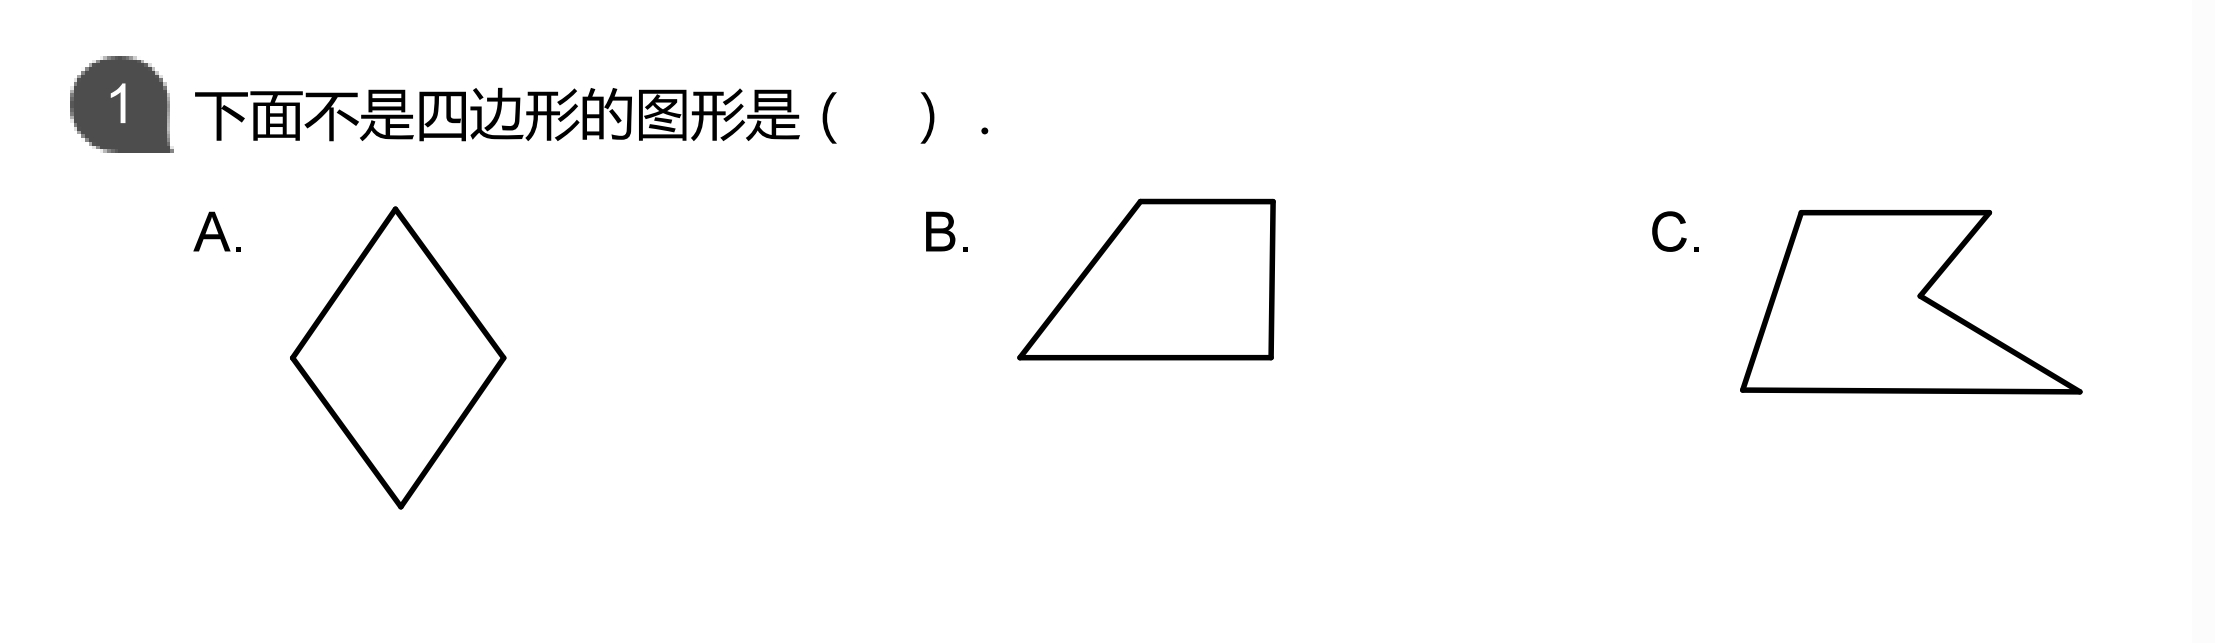
\includegraphics[width=0.4\textwidth]{./pics/Chapter_7/1.png}
%     \end{figure}
%     \vspace{1cm}
%     % 2025数学花园探秘笔试小中年级决赛C卷(B5试卷版).pdf;16934
% }

\item {
    【数字谜】
    下面的算式中,相同的汉字代表相同的数字,不同的汉字代表不同的数字,那么,\\ \myoverline{龙行天下}  表示的四位数是\underline{\hbox to 20mm{}}.
    \begin{figure}[H] 
        \centering
        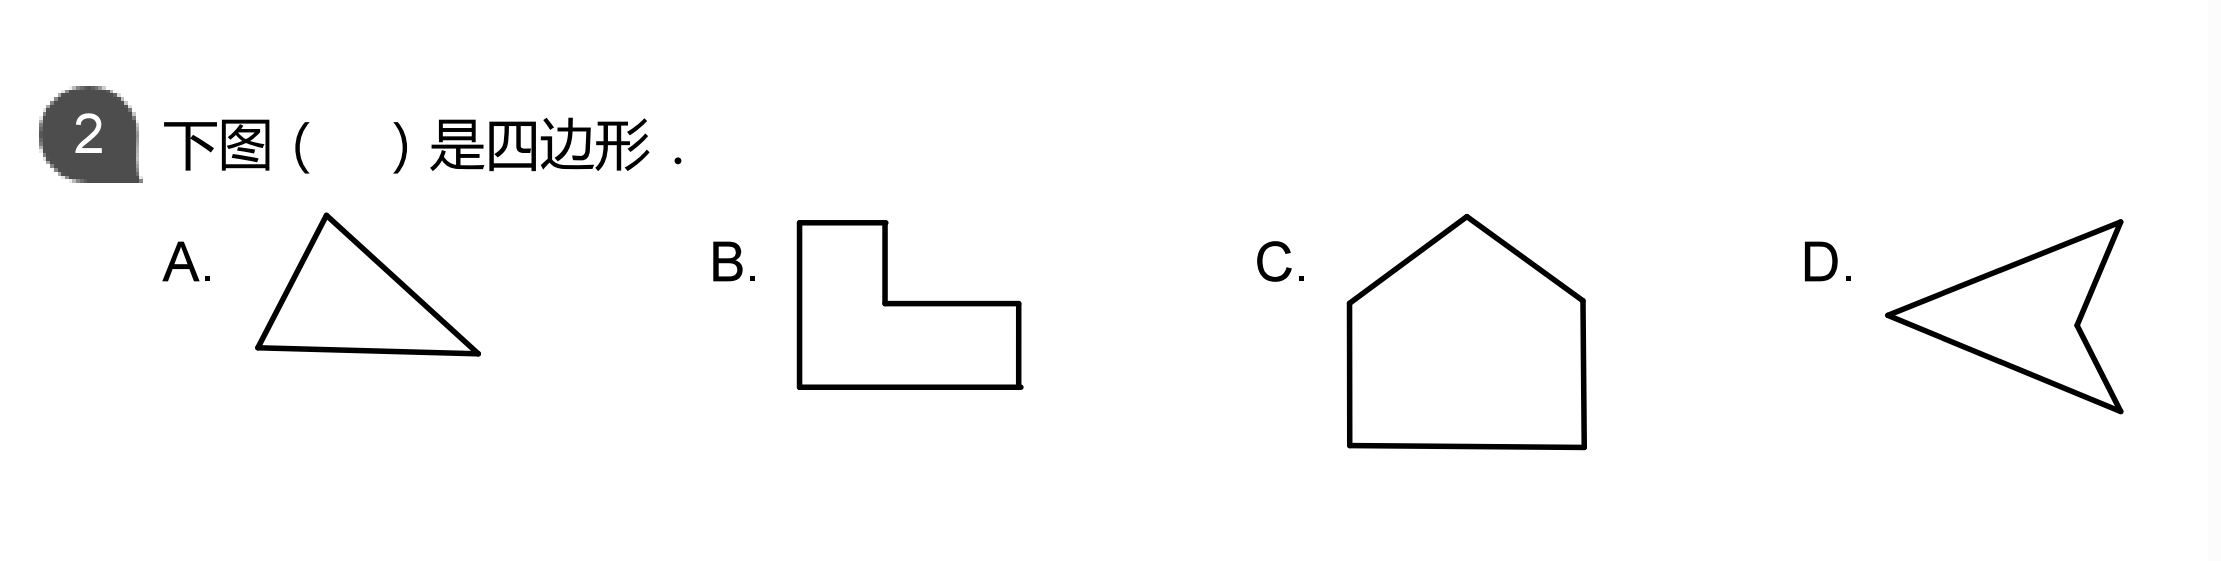
\includegraphics[width=0.4\textwidth]{./pics/Chapter_7/2.png}
    \end{figure}
    \vspace{1cm}
    % 2024
}

\item {
    【数字谜】
    将 $1\sim 9$分别填入到右图的方框中,每个数字用一次,使得竖式成立;现在数字 6、7、8已经被填入,那么竖式的和是\underline{\hbox to 20mm{}}.
    \zihao{2}
    \[
    \begin{array}{r@{\,}r@{}c@{}l}
    & \square & \square & \square \\
    + & \square  & \boxed{7} & \boxed{6} \\
    \cline{1-4}
    & \boxed{8} & \square & \square \\
    \end{array}
    \]
    % \begin{figure}[H] 
    %     \centering
    %     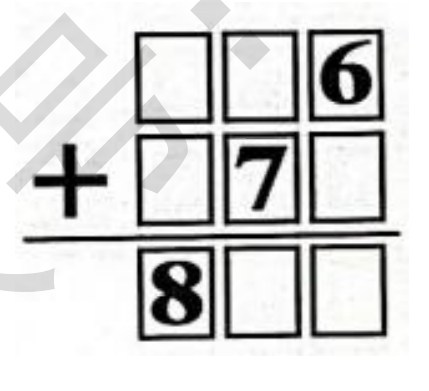
\includegraphics[width=0.3\textwidth]{./pics/Chapter_7/3.png}
    % \end{figure}
    \vspace{1cm}
    % 2023YCB初赛真题答案小中.pdf; 819
    % 改
}

\item {
    【数字谜】
    在右图的加法竖式中,6个汉字恰好代表6个连续的数字,那么,``花园探秘'' 所代表的四位数是\underline{\hbox to 20mm{}}.
    \begin{figure}[H] 
        \centering
        
\includegraphics[width=0.4\textwidth]{./pics/Chapter_7/12.png}
    \end{figure}
    \vspace{1cm}
    % 2021; 8354
}

\item {
    【数字谜】
    在右面的乘法竖式中,相同的汉字代表相同的数字,不同的汉字代表不同的数字;那么,\myoverline{迎接夏天} 代表的四位数是\underline{\hbox to 20mm{}}.
    \begin{figure}[H] 
        \centering
        
\includegraphics[width=0.4\textwidth]{./pics/Chapter_7/14.png}
    \end{figure}
    \vspace{1cm}
    % 2021,迎春杯四年级真题.pdf; 1024
}
		
	\begin{frame}
		\Huge{\centerline{(结束)}}
	\end{frame}
	%------------------------------------------------
	% \subsection{Subsection Example 2}
	
	% \begin{frame}
	% 	\frametitle{Bullet Points}
	% 	\begin{itemize}
	% 		\item What we do may be small, but it has a certain character of permanence.
	% 		\item Euclid geometry was as dazzling as first love.
	% 		\item Talk is cheap, solve the PDE.
	% 	\end{itemize}
	% \end{frame}
	
	% %------------------------------------------------
	
	% \begin{frame}
	% 	\frametitle{Blocks of Highlighted Text}
	% 	\begin{block}{Block 1}
	% 		Certainly the best times were when I was alone with mathematics: free of ambition and pretense, and indifferent to the world.
	% 	\end{block}
		
	% 	% \begin{block}{Block 2}
	% 	% 	Wir müssen wissen, Wir werden wissen.
	% 	% \end{block}
		
	% 	\begin{block}{Block 3}
	% 		If people do not believe that mathematics is simple, it is only because they do not realize how complicated life is.	
	% 	\end{block}
	% \end{frame}
	
	% %------------------------------------------------
	
	% \begin{frame}
	% 	\frametitle{Multiple Columns}
	% 	\begin{columns}[c] % The "c" option specifies centered vertical alignment while the "t" option is used for top vertical alignment
			
	% 		\column{.45\textwidth} % Left column and width
	% 		\textbf{Heading}
	% 		\begin{enumerate}
	% 			\item Statement
	% 			\item Explanation
	% 			\item Example
	% 		\end{enumerate}
			
	% 		\column{.5\textwidth} % Right column and width
	% 		Lorem ipsum dolor sit amet, consectetur adipiscing elit. Integer lectus nisl, ultricies in feugiat rutrum, porttitor sit amet augue. Aliquam ut tortor mauris. Sed volutpat ante purus, quis accumsan dolor.
			
	% 	\end{columns}
	% \end{frame}
	
	% %------------------------------------------------
	% \section{Second Section}
	% %------------------------------------------------
	
	% \begin{frame}
	% 	\frametitle{Table}
	% 	\begin{table}
	% 		\begin{tabular}{l l l}
	% 			\toprule
	% 			\textbf{Treatments} & \textbf{Response 1} & \textbf{Response 2}\\
	% 			\midrule
	% 			Treatment 1 & 0.0003262 & 0.562 \\
	% 			Treatment 2 & 0.0015681 & 0.910 \\
	% 			Treatment 3 & 0.0009271 & 0.296 \\
	% 			\bottomrule
	% 		\end{tabular}
	% 		\caption{Table caption}
	% 	\end{table}
	% \end{frame}
	
	% %------------------------------------------------
	
	% \begin{frame}
	% 	\frametitle{Theorem}
	% 	\begin{theorem}[Mass--energy equivalence]
	% 	\centerline{$E = mc^2$}
	% 	\end{theorem}
	% \end{frame}
	
	%------------------------------------------------
	
	% \begin{frame}[fragile] % Need to use the fragile option when verbatim is used in the slide
	% 	\frametitle{Verbatim}
	% 	\begin{example}[Theorem Slide Code]
	% 		\begin{verbatim}
	% 			\begin{frame}
	% 			\frametitle{Theorem}
	% 			\begin{theorem}[Mass--energy equivalence]
	% 			$E = mc^2$
	% 			\end{theorem}
	% 			\end{frame}
	% 		\end{verbatim}
	% 	\end{example}
	% \end{frame}

\end{document}
